%Exp 1-1
\newcommand{\comment}[1]{}
\chapter{Intro to Labs and Uncertainty}
\label{chap:excel}
\section{Introduction}

There is no such thing as a perfect measurement. All measurements have errors and uncertainties, no matter how hard we might try to minimize them. Understanding possible errors is an important issue in any experimental science. The conclusions we draw from the data, and especially the strength of those conclusions, will depend on how well we control the uncertainties. \myskip

Let's consider an \emph{example}: You're trying to measure something and from theory, you know the expected value should be 2.3. You make two measurements and get two very different values: 2.5 and 1.5. We can see immediately that 2.5 is rather close to the expected value while 1.5 is quite far off. However, we have not taken error into account. Each measurement has a certain amount of uncertainty, or wiggle room. Basically, there's an interval surrounding your measurement where the true value is expected to lie. If your measurements give experimental uncertainties of 0.1 and 1.0 respectively, the new measured values may be expressed $2.5\pm 0.1$ and $1.5\pm 1.0$. The expected value falls within the range of the second measurement, but not the first! \myskip

Analyzing data and error in experiments is essential in making conclusions about the physical laws we are testing. The advent of computers and software made to manipulate large data sets has revolutionized scientist's ability to make conclusions from experimental data. In this lab course, we will be using Microsoft Excel to record data sets from the experiments and determine experimental uncertainties in calculated quantities. We will learn to use excel to propagate uncertainties and plot error bars with our data. You can download a personal copy of Microsoft Excel with your student email address from
\href{https://products.office.com/en-us/student?ms.officeurl=getoffice365}{Office 365 Education} \footnote{https://products.office.com/en-us/student?ms.officeurl=getoffice365}. Please note the sections introducing new Excel tools pertain to the newest version of Excel. If you are using a personal laptop with a different version of Excel, you are responsible for adapting the instructions to your version of Excel. \myskip

The purpose of this introduction is to give some basic information about statistics and uncertainty. The techniques studied here will be essential for the rest of this two-semester lab course. These tools are important in order to arrive at good judgments in any field (like medicine) in which it is necessary to understand not just numerical results, but the uncertainties associated with those results.

\section{Theory}

\subsection{Types of Uncertainties}

Uncertainty in a measurement can arise from three possible origins: the measuring device, the procedure of how you measure, and the observed quantity itself. Usually the largest of these will determine the uncertainty in your data. \myskip

Uncertainties can be divided into two different types: systematic uncertainties and random (statistical) uncertainties\footnote{If you were to engage in further research, random uncertainty is typically referred to as statistical uncertainty.}.

\subsubsection{Systematic Uncertainties}


Systematic uncertainties or systematic errors always bias results in one specific direction. They will cause your measurement to consistently be higher or lower than the accepted value. \myskip

An \emph{example} of a systematic error follows. Assume you want to measure the length of a table in cm using a meter stick. However, the stick is made of metal that has contracted due to the temperature in the room, so that it is less than one meter long. Therefore, all the intervals on the stick are smaller than they should be. Your numerical value for the length of the table will then always be larger than its actual length no matter how often or how carefully you measure. Another example might be measuring temperature using a mercury thermometer in which a bubble is present in the mercury column. \myskip

Systematic errors are usually due to imperfections in the equipment, improper or biased observation, or the presence of additional physical effects not taken into account. (An example might be an experiment on forces and acceleration in which there is friction in the setup and it is not taken into account!) \myskip

In performing experiments, try to estimate the effects of as many systematic errors as you can, and then remove or correct for the most important. By being aware of the sources of systematic error beforehand, it is often possible to perform experiments with sufficient care to compensate for weaknesses in the equipment.

\subsubsection{Random Uncertainties}

In contrast to systematic uncertainties, random uncertainties are an unavoidable result of measurement, no matter how well designed and calibrated the tools you are using. Whenever more than one measurement is taken, the values obtained will not be equal but will exhibit a spread around a mean value, which is considered the most reliable measurement. That spread is known as the random uncertainty. Random uncertainties are unbiased -- meaning it is equally likely that an individual measurement is too high or too low. \myskip

From your everyday experience you might be thinking, ``Stop! Whenever I measure the length of a table with a meter stick I get exactly the same value no matter how often I measure it!''   This may happen if your meter stick is insensitive to random measurements, because you use a coarse scale (like $\mathrm{mm}$) and you always read the length to the nearest $\mathrm{mm}$. But if you would use a meter stick with a finer scale, or if you interpolate to fractions of a millimeter, you would definitely see the spread. As a general rule, if you do not get a spread in values, you can improve your measurements by using a finer scale or by interpolating between the finest scale marks on the ruler. \myskip

How can one reduce the effect of random uncertainties?  Consider the following \emph{example}. Ten people measure the time of a sprinter using stopwatches. It is very unlikely that each of the ten stopwatches will show exactly the same result. Even if all of the people started their watches at exactly the same time (unlikely) some of the people will have stopped the watch early, and others may have done so late. You will observe a spread in the results. If you \emph{average} the times obtained by all ten stop watches, the \emph{mean} value will be a better estimate of the true value than any individual measurement, since the uncertainty we are describing is random, the effects of the people who stop early will compensate for those who stop late. In general, making multiple measurements and averaging can reduce the effect of random uncertainty. \myskip

\emph{Remark}: We usually specify any measurement by including an estimate of the random uncertainty. (Since the random uncertainty is unbiased we note it with a $\pm$ sign). So if we measure a time of 7.6 seconds, but we expect a spread of about 0.2 seconds, we write as a result:
\begin{equation}
    t = (7.6\pm 0.2)\,\mathrm{s}
\end{equation}
indicating that the uncertainty of this measurement is $0.2\,\mathrm{s}$ or about $3\%$. \myskip
\subsection{Accuracy and Precision}
An important distinction in physics is the difference between the {\it{accuracy}} and the {\it{precision }} of a measurement.
Accuracy refers to the closeness of a measured value to a standard or known value. For example, if in lab you obtain a weight measurement of 3.2 kg for a given substance, but the actual or known weight is 10 kg, then your measurement is not accurate. In this case, your measurement is not close to the known value. \myskip

Precision refers to the closeness of two or more measurements to each other. Using the example above, if you weigh a given substance five times, and get 3.2 kg each time, then your measurement is very precise. Precision is independent of accuracy. You can be very precise but inaccurate, as described above. You can also be accurate but imprecise. \myskip

For example, if on average, your measurements for a given substance are close to the known value, but the measurements are far from each other, then you have accuracy without precision. \myskip

A good analogy for understanding accuracy and precision is to imagine a basketball player shooting baskets. If the player shoots with accuracy, his aim will always take the ball close to or into the basket. If the player shoots with precision, his aim will always take the ball to the same location which may or may not be close to the basket. A good player will be both accurate and precise by shooting the ball the same way each time and each time making it in the basket.
\subsection{Numerical Estimates of Uncertainties}

For this laboratory, we will estimate uncertainties with three approximation techniques, which we describe below. You should note which technique you are using in a particular experiment.

\subsubsection{Upper Bound}

Most of our measuring devices in this lab have scales that are coarser than the ability of our eyes to measure.

\begin{figure}[h]
    \begin{center}
        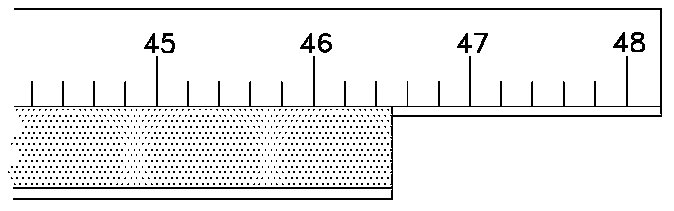
\includegraphics[width=0.5\textwidth]{./Exp1-2/pic/image1.png}
    \end{center}
    \caption{Measuring Length}
    \label{fig:measure}
\end{figure}

For example in the figure above, where we are measuring the length of an object against a meter stick marked in cm, we can definitely say that our result is somewhere between $46.4\,\mathrm{cm}$ and $46.6\,\mathrm{cm}$. We assume as an \emph{upper} bound of our uncertainty, an amount equal to \emph{half} this width (in this case $0.1\,\mathrm{cm}$). The final result can be written as:
\begin{equation}
    \ell = (46.5\pm 0.1)\,\mathrm{cm}
\end{equation}

There will be many circumstances when the error is more complicated than simply the coarseness of the measuring tool. For example, if you find yourself measuring something that is very long or hard to line up properly with a meter stick. In this case, you may need to use some judgement of the best possible measurement to make and the uncertainty will be greater than the millimeter precision of your meter stick. \textbf{It is always best to slightly overestimate error and allow yourself some wiggle room if you feel that better represents your measurement!}

\subsubsection{Estimation from the Spread (2/3 method)} \label{sssec:twothirds}

For data in which there is random uncertainty, we usually observe individual measurements to cluster around the mean and drop in frequency as the values get further from the mean (in both directions).\footnote{There is a precise mathematical procedure to obtain uncertainties (standard deviations) from a number of measured values. Here we will apply a simple ``rule of thumb'' that avoids the more complicated mathematics of that technique. The uncertainty using the standard deviation for the group of values in our example below is 0.2.}  Find the interval around the mean that contains about 2/3 of the measured points: \emph{half} the size of this interval is a good estimate of the uncertainty in each measurement. \myskip

The reasons for choosing a range that includes 2/3 of the values come from the underlying statistics of the normal (or Gaussian) distribution (see figure \ref{fig:bellcurve}). This choice allows us to accurately add and multiply values with errors and has the advantage that the range is not affected much by outliers and occasional mistakes. A range that always includes all of the values is generally less meaningful. \myskip

\emph{Example}: You measure the following values of a specific quantity:
\begin{equation*}
    9.7,\:9.8,\:10,\:10.1,\:10.1,\:10.3
\end{equation*}
The mean of these six values is 10.0. The interval from 9.8 to 10.1 includes 4 of the 6 values; we therefore estimate the uncertainty to be 0.15. The result is that the best estimate of the quantity is 10.0 and the uncertainty of a single measurement is 0.2.\footnote{Note that about 5\% of the measured values will lie \emph{outside} $\pm$ twice the uncertainty}\footnote{While the above method for calculating uncertainty is good enough for our purposes, it oversimplifies a bit the task of calculating the uncertainty of the \emph{mean} of a quantity.  For those who are interested, please see the appendix for elaboration and clarification. }

\subsubsection{Square-Root Estimation in Counting}

For inherently random phenomena that involve counting individual events or occurrences, we measure only a single number $N$. This kind of measurement is relevant to counting the number of radioactive decays in a specific time interval from a sample of material, for example. It is also relevant to counting the number of left-handed people in a random sample of the population. The (absolute) uncertainty of such a single measurement, $N$, is estimated as the square root of $N$ (a counting measurement is expressed as $N \pm \sqrt{N}$). As an example, if we measure 50 radioactive decays in 1 second we should present the result as $50\pm 7$ decays per second. (The quoted uncertainty indicates that a subsequent measurement performed identically could easily result in numbers differing by 7 from 50.)

\subsection{Relative and Absolute Uncertainty}

There are two ways to record uncertainties: the absolute value of the uncertainty or the uncertainty relative to the mean value. So in the example above, you can write $c = (5.1 \pm 0.3)\,\mathrm{cm}$ or equally well $c = 5.1\,\mathrm{cm}\; (1.00 \pm 0.06)$. You can see that if you multiply out the second form you will obtain the first, since $5.1 \times 0.06 = 0.3$. The second form may look a bit odd, but it tells you immediately that the uncertainty is 6\% of the measured value. The number $0.3\,\mathrm{cm}$ is the absolute uncertainty and has the same units as the mean value (cm). The 0.06 (or 6\%) is the relative uncertainty and has no units since it is the ratio of two lengths. It's important to use proper notation when describing uncertainty to remove any unwanted ambiguity, so make sure it's clear when you are using relative or absolute errors.

\subsection{Propagation of Uncertainties}

Often, we are not directly interested in a measured value, but we want to use it in a formula to calculate another quantity. In many cases, we measure many of the quantities in the formula and each has an associated uncertainty. We deal here with how to propagate uncertainties to obtain a well-defined uncertainty on a computed quantity.

\subsubsection{Adding/Subtracting Quantities}

When we \textbf{add or subtract} quantities, the combined uncertainty is the \textbf{sum of the absolute uncertainties} of the constituent parts\footnote{The propagation of random uncertainties is actually slightly more complicated, but the procedure outlined here usually represents a good approximation, and it never underestimates the uncertainty. See the appendix for more information.}.

Take as an example measuring the length of a dog. We measure the distance between the left wall and the tail of the dog and subtract the distance from the wall to the dog's nose.
\begin{figure}[h]
    \begin{center}
        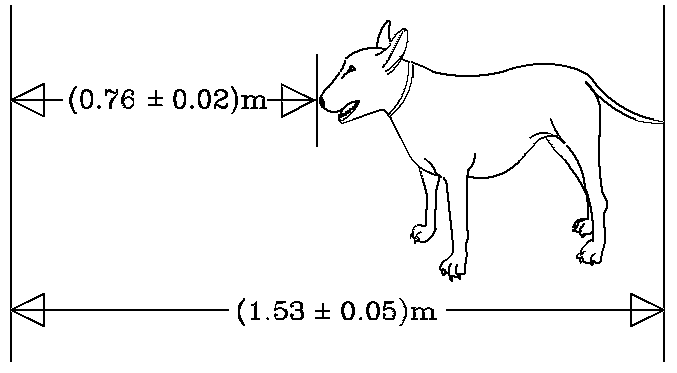
\includegraphics[width=0.5\textwidth]{./Exp1-2/pic/image2.png}
    \end{center}
    \caption{Measuring a Dog}
    \label{fig:dog}
\end{figure}
So the total length of the dog is:
\begin{equation}
    \begin{split}
        \text{Length} &= (1.53\pm 0.05)\,\mathrm{m} - (0.76 \pm 0.02)\,\mathrm{m} \\
        &= \left( 1.53 - 0.76 \right)\pm\left( 0.05 + 0.02 \right)\,\mathrm{m} \\
        &= \left( 0.77 \pm 0.07 \right)\,\mathrm{m}
    \end{split}
\end{equation}

\subsubsection{Multiplying/Dividing Quantities}

When we \textbf{multiply or divide} quantities, the combined \textbf{relative} uncertainty is the \textbf{sum of the relative uncertainties} of the constituent parts.\footnote{Our calculation of the uncertainty actually overestimates it. The correct method does not add the absolute/relative uncertainty, but rather involves evaluating the square root of the sum of the squares. For more information please refer to the appendix of this lab manual.}

Take as an example the area of a rectangle, whose individual sides are measured to be:
\begin{align}
    a = 25.0\pm 0.5\,\mathrm{cm} = 25.0\,\mathrm{cm}\;(1.00\pm 0.02) \nonumber \\
    b = 10.0\pm 0.3\,\mathrm{cm} = 10.0\,\mathrm{cm}\;(1.00\pm 0.03)
\end{align}

The area is obtained as follows:
\begin{equation}
    \begin{split}
        \text{Area} &= \left( 25.0\pm 0.5\,\mathrm{cm} \right)\cdot\left( 10.0\pm 0.3\,\mathrm{cm} \right) \\
        &= 25.0\,\mathrm{cm}\;\left( 1.00\pm 0.02 \right)\cdot 10.0\,\mathrm{cm}\;\left( 1.00\pm 0.03 \right) \\
        &= \left( 25.0\,\mathrm{cm}\cdot 10.0\,\mathrm{cm} \right)\left( 1.00\pm \left( 0.02 + 0.03 \right) \right) \\
        &= 250.0\,\mathrm{cm}^2\;(1.00 \pm 0.05) \\
        &= 250.0\pm 12.5\,\mathrm{cm}^2 \\
        &= 250 \pm 10\,\mathrm{cm}^2
    \end{split}
\end{equation}

Note that the final step has rounded both the result and the uncertainty to an appropriate number of significant digits, given the uncertainty on the lengths of the sides. \myskip

\underline{Remarks:} Note that uncertainties on quantities used in a mathematical relationship always increase the uncertainty on the result. The quantity with the biggest uncertainty usually dominates the final result. Often one quantity will have a much bigger uncertainty than all the others. In such cases, we can simply use this main contribution.

\subsubsection{Multiplication by a Constant}

Multiplying a value by a constant leaves the relative error unchanged. This is equivalent to multiplying the absolute error by the same constant. For example, suppose we are trying to find the circumference of a circle knowing it's radius as $r=1.0 \pm 0.1 \hspace{1mm} \text{cm}$ with error. We would calculate the circumference with error as follows.

\begin{gather}
C = 2\pi r \nonumber \\
 C= 2\pi (1.0 \pm 0.1) \\
 C=6.3 \pm 0.6 \hspace{1mm}  \text{cm} \nonumber
\end{gather}

\subsubsection{Powers and Roots}

When raising a value to a certain power, its \textbf{relative uncertainty is multiplied by the exponent}. This applies to roots as well, since taking the root of a number is equivalent to raising that number to a fractional power.\myskip

Squaring a quantity involves multiplying its relative uncertainty by 2, while cubing a quantity causes its relative uncertainty to be multiplied by 3.\myskip

Taking the square root of a quantity (which is equivalent to raising the quantity to the 1/2 power) causes its relative uncertainty to be multiplied by 1/2. For example, if you know the area of a square to be:
\begin{equation}
    \text{Area} = 100\pm 8\,\mathrm{m^2} = 100\,\mathrm{m}^2\;(1.00\pm 0.08)
\end{equation}
then it follows that the side of the square is:
\begin{equation}
    \text{Side} = 10\,\mathrm{m}\;\left( 1.00\pm 0.04 \right) = 10.0\pm 0.4\,\mathrm{m}
\end{equation}
The most general rule for finding the error in powers and roots is mathematically represented as follows.
\begin{gather}
f(x) = x^n \\
\frac{\sigma_{f(x)}}{f(x)} = |n| \frac{\sigma_x}{x}
\end{gather}
Where $\sigma$ is the {\it{absolute}} uncertainty and $f(x)$ is some power or root of $x$.

\subsubsection{Other Functions}

If you need to calculate the error of a calculation that does not fit into one of these rules (such as trigonometric functions or logarithmic ones), here is a manual method that you can use.\myskip

Based upon the error of the quantity that you determined, you can find the maximum and minimum values of the quantity that you are calculating. The value that you found should be roughly midway between these two quantities. Then if you split the difference between the maximum and minimum you should obtain a reasonable estimate of the error. Mathematically, you would do so as follows.
\begin{gather}
\sigma_{f(x)} = \frac{f(x + \sigma_x) - f(x - \sigma_x)}{2}
\end{gather}

Here is an example: Suppose you measure an angle to be $(47.3 \pm 0.5)^\circ$ and you want to determine the error of $\sin(47.3 \pm 0.5)^\circ$. You find that $\sin(47.3) = 0.735$. Based upon your reported uncertainty, you know that your angle could be as large as $47.8^\circ$ and as small as $46.8^\circ$, and therefore you should calculate $\sin(47.8) = 0.741$ and $\sin(46.8) = 0.729$. So your calculated value is 0.735 but it can be as low as 0.729 and as high as 0.741 and therefore, if you halve the difference between 0.729 and 0.741 you get a reasonable error estimate of 0.006. So you should report your value as $0.735 \pm 0.006$.

\subsection{Best-Fit Line}

In most research laboratories, plotting measurements is found to be the preferred method of reviewing the data and quantitatively measuring the relationship between the experimental variables. This is effective because we often have some idea of the expected relationship between the variables {\it{a priori}}. In these labs, this expected relationship is almost always arranged to be a straight line. But even if we know that the ideal points fit on a precise straight line, experimentally measured data points will not always lie on a single line -- because the measurements always have intrinsic uncertainty. Therefore when the points are plotted, we should include error bars on both axes to indicate the uncertainties in the data. Because real measurements do not all lie on a single straight line, there are a variety of possible lines you might choose to fit the data. \myskip

\begin{figure}[h]
    \begin{center}
        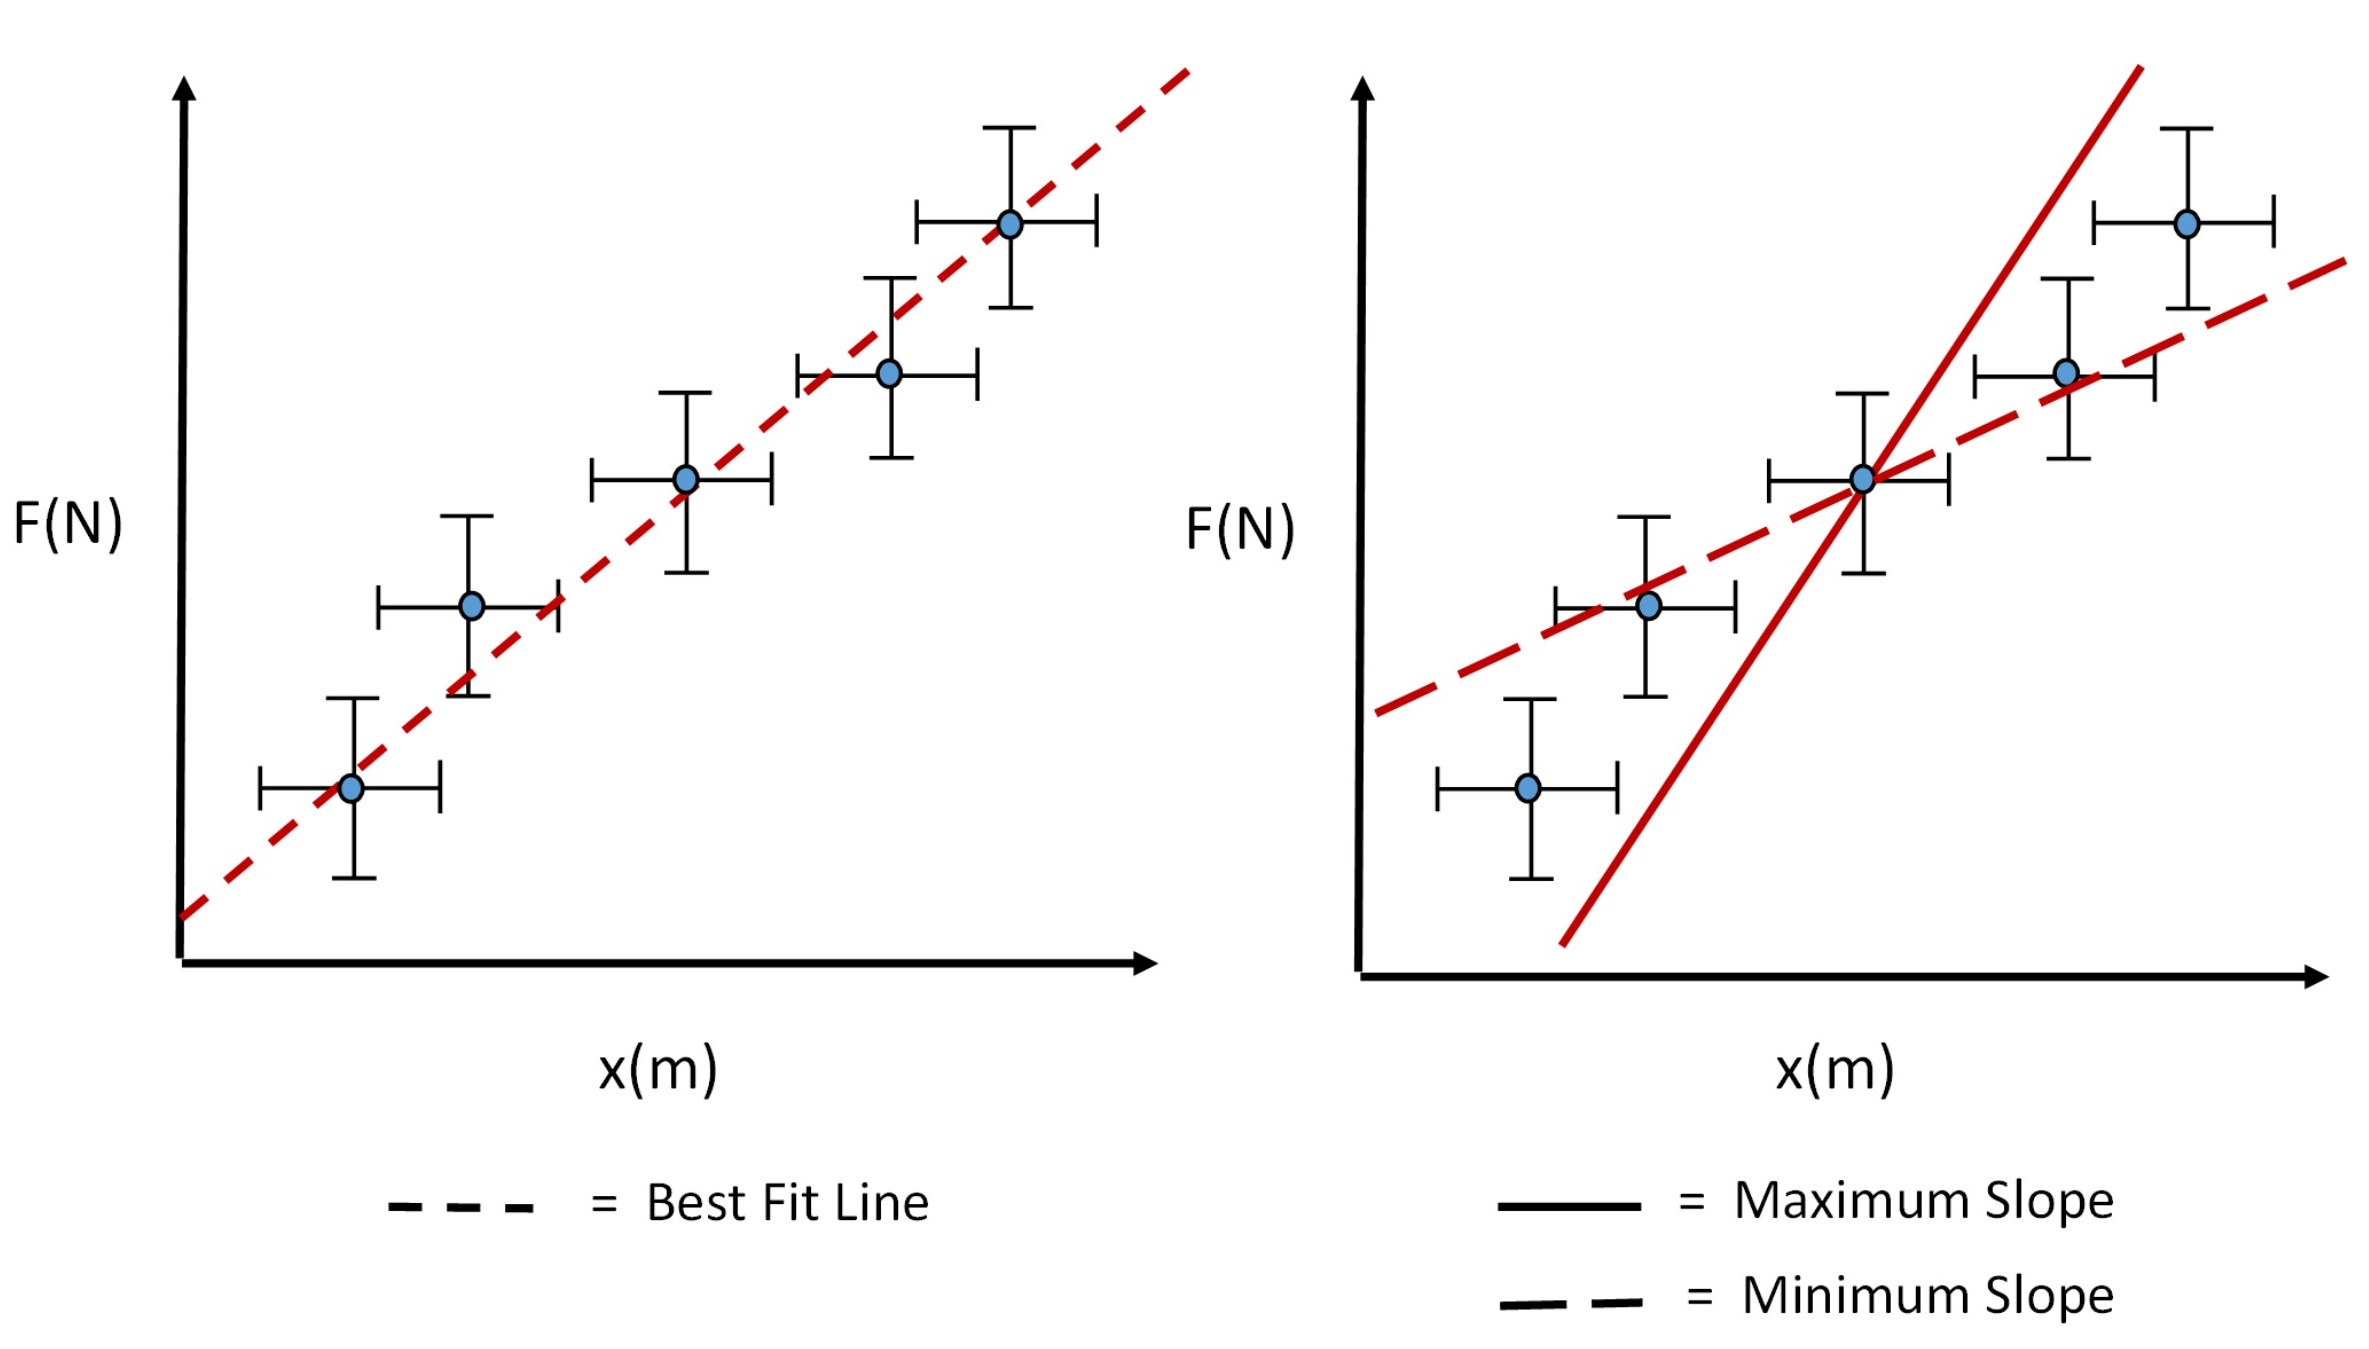
\includegraphics[width=0.9\textwidth, height=0.5\textwidth]{./Exp1-1/pic/image13.jpg}
    \end{center}
    \caption{Left: an example best-fit line. Right: the maximum and minimum possible slope from our data used to calculate uncertainty in the best-fit line. Notice how we have drawn the lines on the outer bounds of the error bars to achieve the maximum and minimum possible slope within the error bars.}
    \label{fig:bestfit}
\end{figure}

How do we know which line represents the best fit? There is an exact mathematical procedure to obtain the best-fit line, but this is usually a very tedious calculation which is outside the scope of this lab. For experiments in this course, you will be using Excel's built-in fitting function for data. The process for doing which will be explained in your next lab. However, if you are interested in learning how to approximate the technique without a computer, please see the appendix.\myskip

\underline{Remark}: Often in our experiments the data points will not look as nice as in the above examples. One or several points may not be close to any best-fit line you try. Such anomalous points may occur, for example, because of a mistake in measuring. In such cases, it is acceptable to ignore these anomalies when estimating the best-fit line (and of course you must note this fact down in your lab report).  Dropping anomalous points must be done with extreme care and only rarely (if you know the point is not physically meaningful).\footnote{More than once, data points that did not behave as theory predicted turned out to be new effects and led to Nobel prizes!}  It is better to choose a line with as many points above the line as below. If you are not sure of your measurements, it is better to re-measure or to take more data points. \myskip

\subsection{Numerical Statistics}
The previous discussions of uncertainty and error tell us how we can quantitatively describe our inability to make perfect single measurements. However, in real physics experiments, very rarely do we draw conclusions from a single data points. As such, it is essential that we know how to quantify error in sets of data. The 2/3 methods as discussed in Section \ref{sssec:twothirds} provides a good estimation of data statistics, but we can more rigorously calculate data set statistics. In statistics, a data set can be well described by the following four fundamental quantities: mean, median, mode, and standard deviation. The mean of a data set is the sum of all numbers in the data set divided by the number of points in the set. It is defined in the following manner.
\begin{gather}
 \text{Average} \equiv \bar x= \sum_{i} \frac{x_i}{N}
\end{gather}
The median of a data set is the middle value in a set of numbers listed in increasing order. The mode is the number that occurs the most number of times in the data set. The standard deviation describes  how the numbers in the data set are distributed around the mean. It is defined as follows.
\begin{gather}
\text{standard deviation} \equiv \sigma = \sqrt{\sum_i \frac{(x_i - \bar x)^2}{N}}
\end{gather}

These four statistical quantities give us enough information to characterize the distribution of our data set. For example, let's consider the two following Data Sets.
\myskip
\begin{center}
\begin{tabular}{c | c | c | c | c | c | c | c | c | c | c | c | c | c  }
&&&&&&&&&&Mean&Median&Mode& $\sigma$ \\
Set 1 & 9&8&11&13&10&10&12&6&9 &9.8&10&10&2.2\\
Set 2 & 11&0&10&40&2&3&10&10&4 &9.8&10&10&11.4
\end{tabular}
\end{center}
\myskip
Notice how both Data Sets have the same mean, median, and mode, which tells us the data points in each set are centered around the mean value of $9.8$. However, the standard deviations are quite different. The large standard deviation in Data Set 2 tells us there must be outliers in the data set which increase the distribution. Whereas, the relatively small standard deviation in the first data set tells us the numbers in set 1 are clustered closely together. Standard deviation is especially important because  it tells us exactly how distributed the number are around the mean value, which gives an indication of how error affects the spread of data points (for example, see figure \ref{fig:bellcurve} for the canonical "bell curve" distribution, also known as the gaussian distribution). The 2/3 method as discussed in Section \ref{sssec:twothirds} is an approximation to the standard deviation since $2/3 \sim 66\%$, which roughly corresponds to the first standard deviation (see figure \ref{fig:bellcurve}).

\begin{figure}[h]
    \begin{center}
        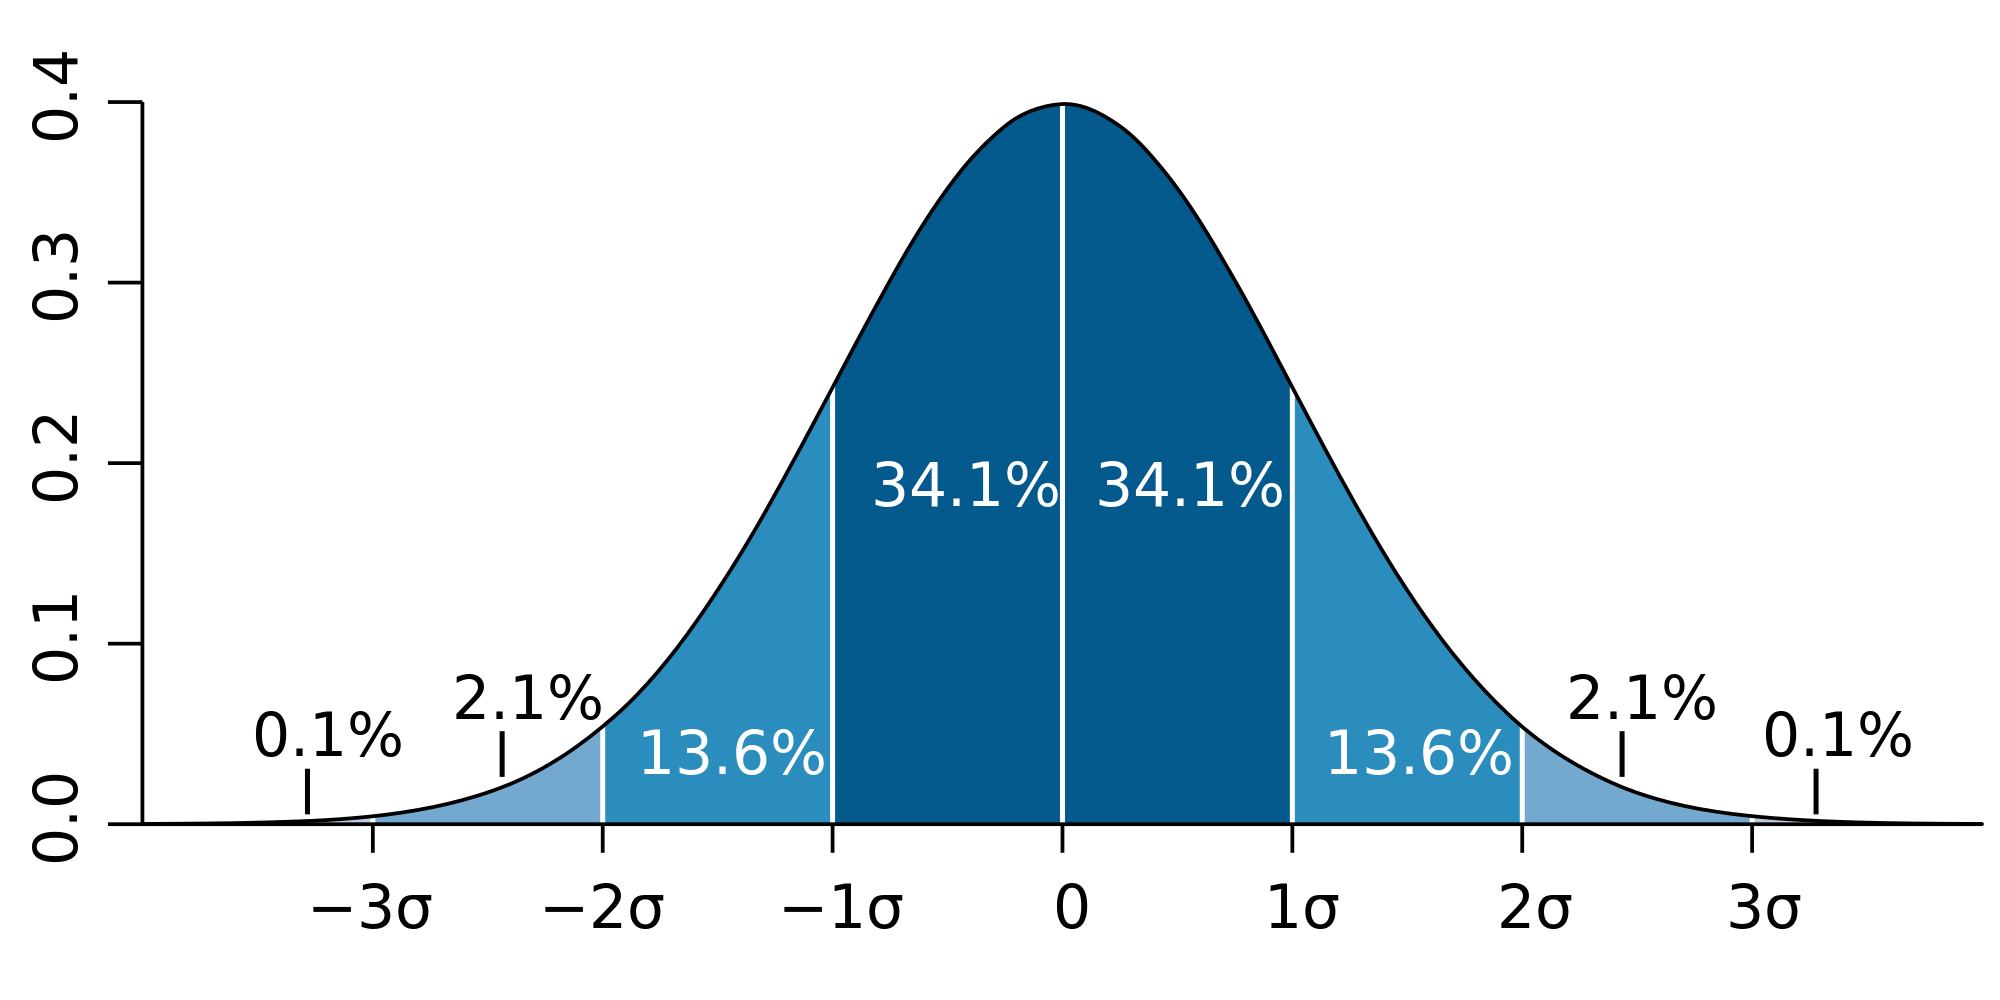
\includegraphics[width=0.7\textwidth]{./Exp1-1/pic/image3.png}
    \end{center}
    \caption{An example of a Gaussian distribution, also known as a bell curve. $\sim 68\%$ of the data points are within 1 standard deviation, $\sim 95\%$ of that data points are contained within 2 standard deviations, $\sim 99.5 \%$ of the data points are contained within 3 standard deviations, etc...}
    \label{fig:bellcurve}
\end{figure}

\subsection{Number of Significant Digits}

The number of significant digits in a result refers to the number of digits that are relevant. The digits may occur after a string of zeroes. For example, the measurement of $2.3\,\mathrm{mm}$ has two significant digits. This does not change if you express the result in meters as $0.0023\,\mathrm{m}$. The number 100.10, by contrast, has 5 significant digits\footnote{Another way to find the number of significant digits is to convert to scientific notation, and count the number of digits in the mantissa (also significand or coefficient). For example: for $1.2\times 10^{2}$, there are two significant digits in $1.2$. }.

When you record a result, you should use the calculated error to determine how many significant digits to keep. Let's illustrate the procedure with the following example. Assume you measure the diameter of a circle to be $d = 1.6232\,\mathrm{cm}$, with an uncertainty of $0.102\,\mathrm{cm}$. You now round your uncertainty to one or two significant digits (up to you). So (using one significant digit) we initially quote $d = (1.6232 \pm 0.1)\,\mathrm{cm}$. Now we compare the mean value with the uncertainty, and keep only those digits that the uncertainty indicates are relevant. Finally, we quote the result as $d = (1.6 \pm 0.1)\,\mathrm{cm}$ for our measurement.

Suppose further that we wish to use this measurement to calculate the circumference $c$ of the circle with the relation $c = \pi\cdot d$. If we use a standard calculator, we might get a 10 digit display indicating:
\begin{equation}
    c = 5.099433195\pm 0.3204424507\,\mathrm{cm}
\end{equation}
This is not a reasonable way to write the result!  The uncertainty in the diameter had only one significant digit, so the uncertainty of the circumference calculated from the diameter cannot be substantially better. Therefore we should record the final result as:
\begin{equation}
    c = 5.1\pm 0.3\,\mathrm{cm}
\end{equation}
(If you do intermediate calculations, it is a good idea to keep as many figures as your calculator can store. The above argument applies when you \underline{record} your results!)

\section{Example Questions}

\myskip
{\bf{Note: Suggested prelab questions are in bold. These will help with conceptual under- standing of the laboratory experiments. }}
\myskip

\noindent \underline{Estimation of Uncertainty}:\myskip

1. You have the following distribution of measured values:
\comment{\begin{table}[h]
    \centering
    \begin{tabular}{|c|l|l|l|}
        \hline
         %& 5 & 10 & 15 \\ \hline
        \quad 0\quad & \hspace{1.5cm} & \hspace{1.5cm} & \hspace{1.5cm} \\ \hline
        \quad 1\quad & I & \hspace{1.5cm} & \hspace{1.5cm} \\ \hline
        \quad 2\quad & III & \hspace{1.5cm} & \hspace{1.5cm} \\ \hline
        \quad 3\quad & IIIII & I & \hspace{1.5cm} \\ \hline
        \quad 4\quad & IIIII & IIII & \hspace{1.5cm} \\ \hline
        \quad 5\quad & IIIII & IIIII & IIIII \\ \hline
        \quad 6\quad & IIIII & IIIII & I \\ \hline
        \quad 7\quad & IIIII & III & \hspace{1.5cm} \\ \hline
        \quad 8\quad & IIII & \hspace{1.5cm} & \hspace{1.5cm} \\ \hline
        \quad 9\quad & II & \hspace{1.5cm} & \hspace{1.5cm} \\ \hline
        \quad 10\quad & I & \hspace{1.5cm} & \hspace{1.5cm} \\ \hline
    \end{tabular}
\end{table}}

$$\begin{array}{ l l }
	1 & (1)\\
	2, 2, 2 & (3)\\
	3, 3, 3, 3, 3, 3 & (6) \\
	4, 4, 4, 4, 4, 4, 4, 4, 4 & (9) \\
	5, 5, 5, 5, 5, 5, 5, 5, 5, 5, 5, 5, 5, 5, 5 & (15) \\ 
	6, 6, 6, 6, 6, 6, 6, 6, 6, 6, 6  & (11)\\
	7, 7, 7, 7, 7, 7, 7, 7 & (8) \\
	8, 8, 8, 8 & (4) \\
	9, 9 & (2) \\
	10 & (1)
\end{array}$$

Estimate the uncertainty using the 2/3 estimate. \myskip

2. Estimate the mean and uncertainty of the following group of values:
\begin{equation*}
    1.6\,\mathrm{s}, 1.3\,\mathrm{s}, 1.7\,\mathrm{s}, 1.4\,\mathrm{s}, 1.6\,\mathrm{s}, 1.2\,\mathrm{s},
\end{equation*}

3. In a radioactive decay you get 16 counts. What is the absolute uncertainty of the number of counts? What is the relative uncertainty? \myskip

4. In a radioactive decay you get 1600 counts. What is the absolute uncertainty of the number of counts? What is the relative uncertainty? \myskip

{\bf{5. How many counts should you get so that the relative uncertainty is $1\%$ or less? }}\myskip

\noindent \underline{Significant digits}: \myskip

6. How many significant digits has $l = 0.0254\,\mathrm{m}$? \myskip

7. Write $t = 1.25578 \pm 0.1247\,\mathrm{s}$ with two significant digits (in the uncertainty). \myskip

\noindent \underline{Propagation of Uncertainty}: \myskip

{\bf{8. For a pendulum with $l = 1.0 \pm 0.1\,\mathrm{m}$, you measure a period of $t = 2.0 \pm 0.2\,\mathrm{s}$. What is the value of the earth's acceleration g?}} \myskip

{\bf{9. You measure the volume of a box by measuring the length of the single sides. For the lengths of the single sides you get:
\begin{equation*}
    a = 10.0 \pm 0.1\,\mathrm{cm}\qquad    b = 5.0 \pm 0.2\,\mathrm{cm} \qquad c = 7.5 \pm 0.3\,\mathrm{cm}
\end{equation*}
What is the volume of the box (including uncertainty and units) in $\mathrm{cm}^3$? What is the volume of the box in $\mathrm{m}^3$? }}\myskip

10. You measure the following quantities:
\begin{align*}
    A &= 1.0 \pm 0.2\,\mathrm{m}\quad B = 2.0 \pm 0.2\,\mathrm{m}\quad        C = 2.5 \pm 0.5\,\mathrm{m/s} \\
    D &= 0.10\pm 0.01\,\mathrm{s}\quad E = 100\pm 10\,\mathrm{m/s^2} &
\end{align*}
Calculate the mean and uncertainty of:
\begin{enumerate}[a)]
    \item $A+B=$
    \item $A-B=$
    \item $C\cdot D=$
    \item $C/D=$
    \item $C\cdot D + A=$
    \item $\frac{1}{2}E\cdot D + C=$
    \item $A\cdot B/(A-B)=$
\end{enumerate}
Include units! For e)--g) perform it step by step.\myskip

\noindent \underline{Relative and Absolute Uncertainty}:\myskip

11. What is the relative uncertainty for $v = 12.25 \pm 0.25\,\mathrm{m/s}$?\myskip

12. What is the absolute uncertainty if the mean value is $120\,\mathrm{s}$ and the relative uncertainty is $5\%$?\myskip

{\bf{13. Given the following measurements, which one has the highest absolute uncertainty and which one has the highest relative uncertainty?}}
\begin{align*}
    l &= 10.0 \pm 0.2\,\mathrm{m} \quad   l = 10.0\,\mathrm{m}\: (1.00 \pm 0.03)   \\
    l &= 7.24\,\mathrm{m}\: (1.00 \pm 0.04) \quad l = 12.5 \pm 0.25\,\mathrm{m}
\end{align*}

14. Given the following measurements which one has the highest absolute uncertainty and which one has the highest relative uncertainty?\myskip
\begin{align*}
    l &= 10.0\pm 0.2\,\mathrm{m} \quad t = 7.5\pm 0.2\,\mathrm{s} \\
    d &= 5.6\,\mathrm{cm}\:(1.00\pm 0.04) \quad v = 6.4\times 10^6\,\mathrm{m/s}\:(1.00\pm 0.03)
\end{align*}
\emph{Caution}: Don't get tricked!\myskip

\noindent \underline{Explanations}:\myskip

{\bf{15. Explain, using your own words, why the uncertainty decreases as you average over several measurements (you might want to take a look at the appendix).}} \myskip

%16. Explain, using your own words, the difference between uncertainty and error as you perform several measurements and average.\myskip

16. You measure the speed of light and get as a result $c = (2.25 \pm 0.25)\times 10^8\,\mathrm{m/s}$. The value you find in books is $c = 299\, 792\, 458\,\mathrm{m/s}$.  Using these values explain the difference between the uncertainty of your measurement and its error!
